\documentclass[1p]{elsarticle_modified}
%\bibliographystyle{elsarticle-num}

%\usepackage[colorlinks]{hyperref}
%\usepackage{abbrmath_seonhwa} %\Abb, \Ascr, \Acal ,\Abf, \Afrak
\usepackage{amsfonts}
\usepackage{amssymb}
\usepackage{amsmath}
\usepackage{amsthm}
\usepackage{scalefnt}
\usepackage{amsbsy}
\usepackage{kotex}
\usepackage{caption}
\usepackage{subfig}
\usepackage{color}
\usepackage{graphicx}
\usepackage{xcolor} %% white, black, red, green, blue, cyan, magenta, yellow
\usepackage{float}
\usepackage{setspace}
\usepackage{hyperref}

\usepackage{tikz}
\usetikzlibrary{arrows}

\usepackage{multirow}
\usepackage{array} % fixed length table
\usepackage{hhline}

%%%%%%%%%%%%%%%%%%%%%
\makeatletter
\renewcommand*\env@matrix[1][\arraystretch]{%
	\edef\arraystretch{#1}%
	\hskip -\arraycolsep
	\let\@ifnextchar\new@ifnextchar
	\array{*\c@MaxMatrixCols c}}
\makeatother %https://tex.stackexchange.com/questions/14071/how-can-i-increase-the-line-spacing-in-a-matrix
%%%%%%%%%%%%%%%

\usepackage[normalem]{ulem}

\newcommand{\msout}[1]{\ifmmode\text{\sout{\ensuremath{#1}}}\else\sout{#1}\fi}
%SOURCE: \msout is \stkout macro in https://tex.stackexchange.com/questions/20609/strikeout-in-math-mode

\newcommand{\cancel}[1]{
	\ifmmode
	{\color{red}\msout{#1}}
	\else
	{\color{red}\sout{#1}}
	\fi
}

\newcommand{\add}[1]{
	{\color{blue}\uwave{#1}}
}

\newcommand{\replace}[2]{
	\ifmmode
	{\color{red}\msout{#1}}{\color{blue}\uwave{#2}}
	\else
	{\color{red}\sout{#1}}{\color{blue}\uwave{#2}}
	\fi
}

\newcommand{\Sol}{\mathcal{S}} %segment
\newcommand{\D}{D} %diagram
\newcommand{\A}{\mathcal{A}} %arc


%%%%%%%%%%%%%%%%%%%%%%%%%%%%%5 test

\def\sl{\operatorname{\textup{SL}}(2,\Cbb)}
\def\psl{\operatorname{\textup{PSL}}(2,\Cbb)}
\def\quan{\mkern 1mu \triangleright \mkern 1mu}

\theoremstyle{definition}
\newtheorem{thm}{Theorem}[section]
\newtheorem{prop}[thm]{Proposition}
\newtheorem{lem}[thm]{Lemma}
\newtheorem{ques}[thm]{Question}
\newtheorem{cor}[thm]{Corollary}
\newtheorem{defn}[thm]{Definition}
\newtheorem{exam}[thm]{Example}
\newtheorem{rmk}[thm]{Remark}
\newtheorem{alg}[thm]{Algorithm}

\newcommand{\I}{\sqrt{-1}}
\begin{document}

%\begin{frontmatter}
%
%\title{Boundary parabolic representations of knots up to 8 crossings}
%
%%% Group authors per affiliation:
%\author{Yunhi Cho} 
%\address{Department of Mathematics, University of Seoul, Seoul, Korea}
%\ead{yhcho@uos.ac.kr}
%
%
%\author{Seonhwa Kim} %\fnref{s_kim}}
%\address{Center for Geometry and Physics, Institute for Basic Science, Pohang, 37673, Korea}
%\ead{ryeona17@ibs.re.kr}
%
%\author{Hyuk Kim}
%\address{Department of Mathematical Sciences, Seoul National University, Seoul 08826, Korea}
%\ead{hyukkim@snu.ac.kr}
%
%\author{Seokbeom Yoon}
%\address{Department of Mathematical Sciences, Seoul National University, Seoul, 08826,  Korea}
%\ead{sbyoon15@snu.ac.kr}
%
%\begin{abstract}
%We find all boundary parabolic representation of knots up to 8 crossings.
%
%\end{abstract}
%\begin{keyword}
%    \MSC[2010] 57M25 
%\end{keyword}
%
%\end{frontmatter}

%\linenumbers
%\tableofcontents
%
\newcommand\colored[1]{\textcolor{white}{\rule[-0.35ex]{0.8em}{1.4ex}}\kern-0.8em\color{red} #1}%
%\newcommand\colored[1]{\textcolor{white}{ #1}\kern-2.17ex	\textcolor{white}{ #1}\kern-1.81ex	\textcolor{white}{ #1}\kern-2.15ex\color{red}#1	}

{\Large $\underline{12n_{0665}~(K12n_{0665})}$}

\setlength{\tabcolsep}{10pt}
\renewcommand{\arraystretch}{1.6}
\vspace{1cm}\begin{tabular}{m{100pt}>{\centering\arraybackslash}m{274pt}}
\multirow{5}{120pt}{
	\centering
	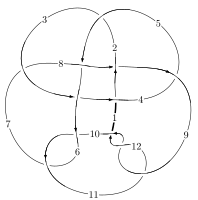
\includegraphics[width=112pt]{../../../GIT/diagram.site/Diagrams/png/2754_12n_0665.png}\\
\ \ \ A knot diagram\footnotemark}&
\allowdisplaybreaks
\textbf{Linearized knot diagam} \\
\cline{2-2}
 &
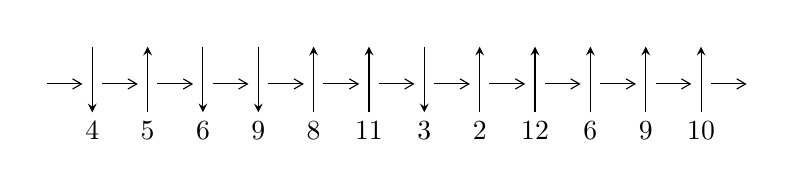
\begin{tikzpicture}[x=20pt, y=17pt]
	% nodes
	\node (C0) at (0, 0) {};
	\node (C1) at (1, 0) {};
	\node (C1U) at (1, +1) {};
	\node (C1D) at (1, -1) {4};

	\node (C2) at (2, 0) {};
	\node (C2U) at (2, +1) {};
	\node (C2D) at (2, -1) {5};

	\node (C3) at (3, 0) {};
	\node (C3U) at (3, +1) {};
	\node (C3D) at (3, -1) {6};

	\node (C4) at (4, 0) {};
	\node (C4U) at (4, +1) {};
	\node (C4D) at (4, -1) {9};

	\node (C5) at (5, 0) {};
	\node (C5U) at (5, +1) {};
	\node (C5D) at (5, -1) {8};

	\node (C6) at (6, 0) {};
	\node (C6U) at (6, +1) {};
	\node (C6D) at (6, -1) {11};

	\node (C7) at (7, 0) {};
	\node (C7U) at (7, +1) {};
	\node (C7D) at (7, -1) {3};

	\node (C8) at (8, 0) {};
	\node (C8U) at (8, +1) {};
	\node (C8D) at (8, -1) {2};

	\node (C9) at (9, 0) {};
	\node (C9U) at (9, +1) {};
	\node (C9D) at (9, -1) {12};

	\node (C10) at (10, 0) {};
	\node (C10U) at (10, +1) {};
	\node (C10D) at (10, -1) {6};

	\node (C11) at (11, 0) {};
	\node (C11U) at (11, +1) {};
	\node (C11D) at (11, -1) {9};

	\node (C12) at (12, 0) {};
	\node (C12U) at (12, +1) {};
	\node (C12D) at (12, -1) {10};
	\node (C13) at (13, 0) {};

	% arrows
	\draw[->,>={angle 60}]
	(C0) edge (C1) (C1) edge (C2) (C2) edge (C3) (C3) edge (C4) (C4) edge (C5) (C5) edge (C6) (C6) edge (C7) (C7) edge (C8) (C8) edge (C9) (C9) edge (C10) (C10) edge (C11) (C11) edge (C12) (C12) edge (C13) ;	\draw[->,>=stealth]
	(C1U) edge (C1D) (C2D) edge (C2U) (C3U) edge (C3D) (C4U) edge (C4D) (C5D) edge (C5U) (C6D) edge (C6U) (C7U) edge (C7D) (C8D) edge (C8U) (C9D) edge (C9U) (C10D) edge (C10U) (C11D) edge (C11U) (C12D) edge (C12U) ;
	\end{tikzpicture} \\
\hhline{~~} \\& 
\textbf{Solving Sequence} \\ \cline{2-2} 
 &
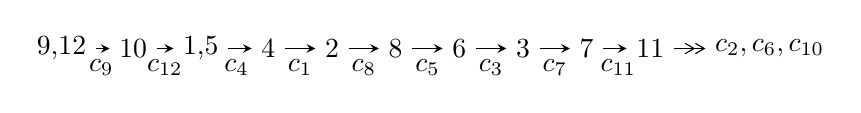
\begin{tikzpicture}[x=23pt, y=7pt]
	% node
	\node (A0) at (-1/8, 0) {9,12};
	\node (A1) at (1, 0) {10};
	\node (A2) at (33/16, 0) {1,5};
	\node (A3) at (25/8, 0) {4};
	\node (A4) at (33/8, 0) {2};
	\node (A5) at (41/8, 0) {8};
	\node (A6) at (49/8, 0) {6};
	\node (A7) at (57/8, 0) {3};
	\node (A8) at (65/8, 0) {7};
	\node (A9) at (73/8, 0) {11};
	\node (C1) at (1/2, -1) {$c_{9}$};
	\node (C2) at (3/2, -1) {$c_{12}$};
	\node (C3) at (21/8, -1) {$c_{4}$};
	\node (C4) at (29/8, -1) {$c_{1}$};
	\node (C5) at (37/8, -1) {$c_{8}$};
	\node (C6) at (45/8, -1) {$c_{5}$};
	\node (C7) at (53/8, -1) {$c_{3}$};
	\node (C8) at (61/8, -1) {$c_{7}$};
	\node (C9) at (69/8, -1) {$c_{11}$};
	\node (A10) at (11, 0) {$c_{2},c_{6},c_{10}$};

	% edge
	\draw[->,>=stealth]	
	(A0) edge (A1) (A1) edge (A2) (A2) edge (A3) (A3) edge (A4) (A4) edge (A5) (A5) edge (A6) (A6) edge (A7) (A7) edge (A8) (A8) edge (A9) ;
	\draw[->>,>={angle 60}]	
	(A9) edge (A10);
\end{tikzpicture} \\ 

\end{tabular} \\

\footnotetext{
The image of knot diagram is generated by the software ``\textbf{Draw programme}" developed by Andrew Bartholomew(\url{http://www.layer8.co.uk/maths/draw/index.htm\#Running-draw}), where we modified some parts for our purpose(\url{https://github.com/CATsTAILs/LinksPainter}).
}\phantom \\ \newline 
\centering \textbf{Ideals for irreducible components\footnotemark of $X_{\text{par}}$} 
 
\begin{align*}
I^u_{1}&=\langle 
1.16371\times10^{21} u^{21}-5.81881\times10^{21} u^{20}+\cdots+1.46625\times10^{23} b-4.63210\times10^{22},\\
\phantom{I^u_{1}}&\phantom{= \langle  }2.23290\times10^{22} u^{21}-1.79700\times10^{23} u^{20}+\cdots+1.17300\times10^{24} a-8.46516\times10^{23},\;u^{22}-7 u^{21}+\cdots- u-16\rangle \\
I^u_{2}&=\langle 
-12 a^3+35 a^2+361 b+258 a+225,\;4 a^4+7 a^3+20 a^2+5 a+11,\;u+1\rangle \\
I^u_{3}&=\langle 
- u^8+4 u^7-6 u^6+2 u^5+5 u^4-6 u^3+4 u^2+b-3 u,\;u^8-3 u^7+2 u^6+4 u^5-7 u^4+u^3+u^2+a+u+2,\\
\phantom{I^u_{3}}&\phantom{= \langle  }u^{11}-4 u^{10}+5 u^9+2 u^8-11 u^7+8 u^6- u^4+4 u^3-5 u^2+u-1\rangle \\
I^u_{4}&=\langle 
-1309 u^{10} a+39316 u^{10}+\cdots-49959 a-27286,\;-16711 u^{10} a+2773 u^{10}+\cdots-53855 a-50795,\\
\phantom{I^u_{4}}&\phantom{= \langle  }u^{11}-5 u^{10}+12 u^9-14 u^8+4 u^7+11 u^6-16 u^5+14 u^4-8 u^3-13 u^2+7 u-1\rangle \\
I^u_{5}&=\langle 
-2 a^5-176 a^4-669 a^3+284 a^2+13805 b+9351 a+7409,\;a^6+6 a^5+21 a^4+39 a^3+66 a^2+49 a+59,\\
\phantom{I^u_{5}}&\phantom{= \langle  }u+1\rangle \\
I^u_{6}&=\langle 
a u+b- a-2 u+3,\;a^2+4 a u-3 a-3 u+6,\;u^2- u-1\rangle \\
\\
\end{align*}
\raggedright * 6 irreducible components of $\dim_{\mathbb{C}}=0$, with total 69 representations.\\
\footnotetext{All coefficients of polynomials are rational numbers. But the coefficients are sometimes approximated in decimal forms when there is not enough margin.}
\newpage
\renewcommand{\arraystretch}{1}
\centering \section*{I. $I^u_{1}= \langle 1.16\times10^{21} u^{21}-5.82\times10^{21} u^{20}+\cdots+1.47\times10^{23} b-4.63\times10^{22},\;2.23\times10^{22} u^{21}-1.80\times10^{23} u^{20}+\cdots+1.17\times10^{24} a-8.47\times10^{23},\;u^{22}-7 u^{21}+\cdots- u-16 \rangle$}
\flushleft \textbf{(i) Arc colorings}\\
\begin{tabular}{m{7pt} m{180pt} m{7pt} m{180pt} }
\flushright $a_{9}=$&$\begin{pmatrix}1\\0\end{pmatrix}$ \\
\flushright $a_{12}=$&$\begin{pmatrix}0\\u\end{pmatrix}$ \\
\flushright $a_{10}=$&$\begin{pmatrix}1\\- u^2\end{pmatrix}$ \\
\flushright $a_{1}=$&$\begin{pmatrix}u\\- u^3+u\end{pmatrix}$ \\
\flushright $a_{5}=$&$\begin{pmatrix}-0.0190358 u^{21}+0.153197 u^{20}+\cdots+2.30959 u+0.721667\\-0.00793664 u^{21}+0.0396850 u^{20}+\cdots+0.0736575 u+0.315914\end{pmatrix}$ \\
\flushright $a_{4}=$&$\begin{pmatrix}-0.0269724 u^{21}+0.192882 u^{20}+\cdots+2.38324 u+1.03758\\-0.00793664 u^{21}+0.0396850 u^{20}+\cdots+0.0736575 u+0.315914\end{pmatrix}$ \\
\flushright $a_{2}=$&$\begin{pmatrix}-0.00755456 u^{21}+0.0556100 u^{20}+\cdots+2.97731 u+1.14656\\0.0129445 u^{21}-0.0689040 u^{20}+\cdots+0.462289 u+0.147994\end{pmatrix}$ \\
\flushright $a_{8}=$&$\begin{pmatrix}0.0468616 u^{21}-0.281682 u^{20}+\cdots+0.728053 u+0.542790\\-0.0303212 u^{21}+0.179358 u^{20}+\cdots-0.268846 u-0.786470\end{pmatrix}$ \\
\flushright $a_{6}=$&$\begin{pmatrix}-0.0501899 u^{21}+0.326221 u^{20}+\cdots+0.776174 u-0.236818\\0.0251088 u^{21}-0.165046 u^{20}+\cdots+0.287008 u+0.803039\end{pmatrix}$ \\
\flushright $a_{3}=$&$\begin{pmatrix}-0.0503171 u^{21}+0.321861 u^{20}+\cdots+0.00116367 u-0.311783\\0.0264975 u^{21}-0.160879 u^{20}+\cdots+1.44637 u+0.689429\end{pmatrix}$ \\
\flushright $a_{7}=$&$\begin{pmatrix}0.0529780 u^{21}-0.337734 u^{20}+\cdots-0.360484 u+0.467102\\-0.0278969 u^{21}+0.176559 u^{20}+\cdots-0.702698 u-1.03332\end{pmatrix}$ \\
\flushright $a_{11}=$&$\begin{pmatrix}- u\\u\end{pmatrix}$\\&\end{tabular}
\flushleft \textbf{(ii) Obstruction class $= -1$}\\~\\
\flushleft \textbf{(iii) Cusp Shapes $= \frac{1046540992390926455030041}{4692001596758932331121536} u^{21}-\frac{692312832330241174483901}{586500199594866541390192} u^{20}+\cdots+\frac{21996001093684558786173143}{4692001596758932331121536} u+\frac{1233054846153246715242967}{293250099797433270695096}$}\\~\\
\newpage\renewcommand{\arraystretch}{1}
\flushleft \textbf{(iv) u-Polynomials at the component}\newline \\
\begin{tabular}{m{50pt}|m{274pt}}
Crossings & \hspace{64pt}u-Polynomials at each crossing \\
\hline $$\begin{aligned}c_{1},c_{3}\end{aligned}$$&$\begin{aligned}
&u^{22}-22 u^{20}+\cdots-78 u+1
\end{aligned}$\\
\hline $$\begin{aligned}c_{2}\end{aligned}$$&$\begin{aligned}
&u^{22}+17 u^{21}+\cdots+72 u+4
\end{aligned}$\\
\hline $$\begin{aligned}c_{4},c_{7}\end{aligned}$$&$\begin{aligned}
&u^{22}-10 u^{20}+\cdots-82 u+17
\end{aligned}$\\
\hline $$\begin{aligned}c_{5},c_{8}\end{aligned}$$&$\begin{aligned}
&u^{22}+u^{21}+\cdots- u+1
\end{aligned}$\\
\hline $$\begin{aligned}c_{6},c_{10}\end{aligned}$$&$\begin{aligned}
&u^{22}+5 u^{21}+\cdots+224 u-256
\end{aligned}$\\
\hline $$\begin{aligned}c_{9},c_{11},c_{12}\end{aligned}$$&$\begin{aligned}
&u^{22}+7 u^{21}+\cdots+u-16
\end{aligned}$\\
\hline
\end{tabular}\\~\\
\newpage\renewcommand{\arraystretch}{1}
\flushleft \textbf{(v) Riley Polynomials at the component}\newline \\
\begin{tabular}{m{50pt}|m{274pt}}
Crossings & \hspace{64pt}Riley Polynomials at each crossing \\
\hline $$\begin{aligned}c_{1},c_{3}\end{aligned}$$&$\begin{aligned}
&y^{22}-44 y^{21}+\cdots-6066 y+1
\end{aligned}$\\
\hline $$\begin{aligned}c_{2}\end{aligned}$$&$\begin{aligned}
&y^{22}- y^{21}+\cdots-984 y+16
\end{aligned}$\\
\hline $$\begin{aligned}c_{4},c_{7}\end{aligned}$$&$\begin{aligned}
&y^{22}-20 y^{21}+\cdots-4038 y+289
\end{aligned}$\\
\hline $$\begin{aligned}c_{5},c_{8}\end{aligned}$$&$\begin{aligned}
&y^{22}+9 y^{21}+\cdots+9 y+1
\end{aligned}$\\
\hline $$\begin{aligned}c_{6},c_{10}\end{aligned}$$&$\begin{aligned}
&y^{22}+27 y^{21}+\cdots-291840 y+65536
\end{aligned}$\\
\hline $$\begin{aligned}c_{9},c_{11},c_{12}\end{aligned}$$&$\begin{aligned}
&y^{22}-5 y^{21}+\cdots- y+256
\end{aligned}$\\
\hline
\end{tabular}\\~\\
\newpage\flushleft \textbf{(vi) Complex Volumes and Cusp Shapes}
$$\begin{array}{c|c|c}  
\text{Solutions to }I^u_{1}& \I (\text{vol} + \sqrt{-1}CS) & \text{Cusp shape}\\
 \hline 
\begin{aligned}
u &= -1.073320 + 0.196864 I \\
a &= -0.633075 + 1.048060 I \\
b &= -0.468525 - 0.581818 I\end{aligned}
 & \phantom{-}0.748660 - 0.578139 I & \phantom{-}4.16300 - 3.21064 I \\ \hline\begin{aligned}
u &= -1.073320 - 0.196864 I \\
a &= -0.633075 - 1.048060 I \\
b &= -0.468525 + 0.581818 I\end{aligned}
 & \phantom{-}0.748660 + 0.578139 I & \phantom{-}4.16300 + 3.21064 I \\ \hline\begin{aligned}
u &= \phantom{-}1.196940 + 0.138834 I \\
a &= \phantom{-}0.69651 - 1.48448 I \\
b &= -0.525572 + 0.904919 I\end{aligned}
 & \phantom{-}4.76890 + 7.93706 I & \phantom{-}14.4936 - 13.4042 I \\ \hline\begin{aligned}
u &= \phantom{-}1.196940 - 0.138834 I \\
a &= \phantom{-}0.69651 + 1.48448 I \\
b &= -0.525572 - 0.904919 I\end{aligned}
 & \phantom{-}4.76890 - 7.93706 I & \phantom{-}14.4936 + 13.4042 I \\ \hline\begin{aligned}
u &= -1.281740 + 0.445541 I \\
a &= -1.340360 - 0.152402 I \\
b &= \phantom{-}1.042560 - 0.544528 I\end{aligned}
 & \phantom{-}0.63415 - 1.82383 I & \phantom{-}3.25206 + 1.96969 I \\ \hline\begin{aligned}
u &= -1.281740 - 0.445541 I \\
a &= -1.340360 + 0.152402 I \\
b &= \phantom{-}1.042560 + 0.544528 I\end{aligned}
 & \phantom{-}0.63415 + 1.82383 I & \phantom{-}3.25206 - 1.96969 I \\ \hline\begin{aligned}
u &= \phantom{-}1.41326\phantom{ +0.000000I} \\
a &= \phantom{-}1.00267\phantom{ +0.000000I} \\
b &= -0.555579\phantom{ +0.000000I}\end{aligned}
 & \phantom{-}7.32600\phantom{ +0.000000I} & \phantom{-}23.7620\phantom{ +0.000000I} \\ \hline\begin{aligned}
u &= -0.583556\phantom{ +0.000000I} \\
a &= -0.207344\phantom{ +0.000000I} \\
b &= -0.336659\phantom{ +0.000000I}\end{aligned}
 & \phantom{-}0.970302\phantom{ +0.000000I} & \phantom{-}10.0070\phantom{ +0.000000I} \\ \hline\begin{aligned}
u &= -0.37029 + 1.42559 I \\
a &= \phantom{-}0.958773 + 0.111950 I \\
b &= -1.88452 + 0.10002 I\end{aligned}
 & -3.47219 - 4.63898 I & \phantom{-}1.76510 + 3.68966 I \\ \hline\begin{aligned}
u &= -0.37029 - 1.42559 I \\
a &= \phantom{-}0.958773 - 0.111950 I \\
b &= -1.88452 - 0.10002 I\end{aligned}
 & -3.47219 + 4.63898 I & \phantom{-}1.76510 - 3.68966 I\\
 \hline 
 \end{array}$$\newpage$$\begin{array}{c|c|c}  
\text{Solutions to }I^u_{1}& \I (\text{vol} + \sqrt{-1}CS) & \text{Cusp shape}\\
 \hline 
\begin{aligned}
u &= \phantom{-}0.305160 + 0.425228 I \\
a &= \phantom{-}0.75251 + 1.97105 I \\
b &= \phantom{-}0.656252 - 0.746018 I\end{aligned}
 & -0.88734 + 1.99220 I & -1.51650 - 2.98007 I \\ \hline\begin{aligned}
u &= \phantom{-}0.305160 - 0.425228 I \\
a &= \phantom{-}0.75251 - 1.97105 I \\
b &= \phantom{-}0.656252 + 0.746018 I\end{aligned}
 & -0.88734 - 1.99220 I & -1.51650 + 2.98007 I \\ \hline\begin{aligned}
u &= \phantom{-}1.01095 + 1.14167 I \\
a &= \phantom{-}0.424540 - 0.460153 I \\
b &= -1.387840 + 0.091887 I\end{aligned}
 & -9.81793 + 5.07725 I & -1.39233 - 9.54863 I \\ \hline\begin{aligned}
u &= \phantom{-}1.01095 - 1.14167 I \\
a &= \phantom{-}0.424540 + 0.460153 I \\
b &= -1.387840 - 0.091887 I\end{aligned}
 & -9.81793 - 5.07725 I & -1.39233 + 9.54863 I \\ \hline\begin{aligned}
u &= \phantom{-}1.16674 + 1.00051 I \\
a &= \phantom{-}0.282150 - 1.116250 I \\
b &= -1.143540 + 0.418541 I\end{aligned}
 & -9.23521 + 2.88093 I & \phantom{-}1.62002 + 2.72235 I \\ \hline\begin{aligned}
u &= \phantom{-}1.16674 - 1.00051 I \\
a &= \phantom{-}0.282150 + 1.116250 I \\
b &= -1.143540 - 0.418541 I\end{aligned}
 & -9.23521 - 2.88093 I & \phantom{-}1.62002 - 2.72235 I \\ \hline\begin{aligned}
u &= -0.238163 + 0.343586 I \\
a &= \phantom{-}0.92161 + 1.69413 I \\
b &= \phantom{-}0.423005 + 0.405652 I\end{aligned}
 & -1.61974 - 1.37202 I & -2.26771 + 5.71937 I \\ \hline\begin{aligned}
u &= -0.238163 - 0.343586 I \\
a &= \phantom{-}0.92161 - 1.69413 I \\
b &= \phantom{-}0.423005 - 0.405652 I\end{aligned}
 & -1.61974 + 1.37202 I & -2.26771 - 5.71937 I \\ \hline\begin{aligned}
u &= \phantom{-}1.44040 + 1.00087 I \\
a &= -0.54794 + 2.42657 I \\
b &= \phantom{-}1.53075 - 1.61655 I\end{aligned}
 & -10.9142 + 15.8777 I & \phantom{-}4.46326 - 7.01203 I \\ \hline\begin{aligned}
u &= \phantom{-}1.44040 - 1.00087 I \\
a &= -0.54794 - 2.42657 I \\
b &= \phantom{-}1.53075 + 1.61655 I\end{aligned}
 & -10.9142 - 15.8777 I & \phantom{-}4.46326 + 7.01203 I\\
 \hline 
 \end{array}$$\newpage$$\begin{array}{c|c|c}  
\text{Solutions to }I^u_{1}& \I (\text{vol} + \sqrt{-1}CS) & \text{Cusp shape}\\
 \hline 
\begin{aligned}
u &= \phantom{-}0.92846 + 1.61543 I \\
a &= -1.69364 - 0.69437 I \\
b &= \phantom{-}2.20355 + 1.18551 I\end{aligned}
 & -13.0092 - 6.5361 I & \phantom{-}2.81617 + 3.19876 I \\ \hline\begin{aligned}
u &= \phantom{-}0.92846 - 1.61543 I \\
a &= -1.69364 + 0.69437 I \\
b &= \phantom{-}2.20355 - 1.18551 I\end{aligned}
 & -13.0092 + 6.5361 I & \phantom{-}2.81617 - 3.19876 I\\
 \hline 
 \end{array}$$\newpage\newpage\renewcommand{\arraystretch}{1}
\centering \section*{II. $I^u_{2}= \langle -12 a^3+35 a^2+361 b+258 a+225,\;4 a^4+7 a^3+20 a^2+5 a+11,\;u+1 \rangle$}
\flushleft \textbf{(i) Arc colorings}\\
\begin{tabular}{m{7pt} m{180pt} m{7pt} m{180pt} }
\flushright $a_{9}=$&$\begin{pmatrix}1\\0\end{pmatrix}$ \\
\flushright $a_{12}=$&$\begin{pmatrix}0\\-1\end{pmatrix}$ \\
\flushright $a_{10}=$&$\begin{pmatrix}1\\-1\end{pmatrix}$ \\
\flushright $a_{1}=$&$\begin{pmatrix}-1\\0\end{pmatrix}$ \\
\flushright $a_{5}=$&$\begin{pmatrix}a\\0.0332410 a^{3}-0.0969529 a^{2}-0.714681 a-0.623269\end{pmatrix}$ \\
\flushright $a_{4}=$&$\begin{pmatrix}0.0332410 a^{3}-0.0969529 a^{2}+0.285319 a-0.623269\\0.0332410 a^{3}-0.0969529 a^{2}-0.714681 a-0.623269\end{pmatrix}$ \\
\flushright $a_{2}=$&$\begin{pmatrix}-0.0332410 a^{3}+0.0969529 a^{2}-0.285319 a-1.37673\\-0.188366 a^{3}-0.783934 a^{2}-0.950139 a-0.468144\end{pmatrix}$ \\
\flushright $a_{8}=$&$\begin{pmatrix}0.443213 a^{3}+1.37396 a^{2}+1.47091 a+1.68975\\-0.221607 a^{3}-0.686981 a^{2}-0.235457 a-0.844875\end{pmatrix}$ \\
\flushright $a_{6}=$&$\begin{pmatrix}0.387812 a^{3}+0.202216 a^{2}+0.662050 a+0.728532\\-0.387812 a^{3}-0.202216 a^{2}-0.662050 a-0.728532\end{pmatrix}$ \\
\flushright $a_{3}=$&$\begin{pmatrix}0.288089 a^{3}+0.493075 a^{2}-0.193906 a-0.401662\\-0.221607 a^{3}-0.686981 a^{2}-0.235457 a-0.844875\end{pmatrix}$ \\
\flushright $a_{7}=$&$\begin{pmatrix}0.387812 a^{3}+0.202216 a^{2}+0.662050 a+0.728532\\-0.387812 a^{3}-0.202216 a^{2}-0.662050 a-0.728532\end{pmatrix}$ \\
\flushright $a_{11}=$&$\begin{pmatrix}1\\-1\end{pmatrix}$\\&\end{tabular}
\flushleft \textbf{(ii) Obstruction class $= 1$}\\~\\
\flushleft \textbf{(iii) Cusp Shapes $= \frac{640}{361} a^3+\frac{1623}{361} a^2+\frac{2846}{361} a+\frac{2079}{361}$}\\~\\
\newpage\renewcommand{\arraystretch}{1}
\flushleft \textbf{(iv) u-Polynomials at the component}\newline \\
\begin{tabular}{m{50pt}|m{274pt}}
Crossings & \hspace{64pt}u-Polynomials at each crossing \\
\hline $$\begin{aligned}c_{1},c_{3},c_{4}\end{aligned}$$&$\begin{aligned}
&u^4+u^2- u+1
\end{aligned}$\\
\hline $$\begin{aligned}c_{2}\end{aligned}$$&$\begin{aligned}
&u^4-3 u^3+4 u^2-3 u+2
\end{aligned}$\\
\hline $$\begin{aligned}c_{5}\end{aligned}$$&$\begin{aligned}
&u^4+2 u^3+3 u^2+u+1
\end{aligned}$\\
\hline $$\begin{aligned}c_{6},c_{10}\end{aligned}$$&$\begin{aligned}
&u^4
\end{aligned}$\\
\hline $$\begin{aligned}c_{7}\end{aligned}$$&$\begin{aligned}
&u^4+u^2+u+1
\end{aligned}$\\
\hline $$\begin{aligned}c_{8}\end{aligned}$$&$\begin{aligned}
&u^4-2 u^3+3 u^2- u+1
\end{aligned}$\\
\hline $$\begin{aligned}c_{9}\end{aligned}$$&$\begin{aligned}
&(u+1)^4
\end{aligned}$\\
\hline $$\begin{aligned}c_{11},c_{12}\end{aligned}$$&$\begin{aligned}
&(u-1)^4
\end{aligned}$\\
\hline
\end{tabular}\\~\\
\newpage\renewcommand{\arraystretch}{1}
\flushleft \textbf{(v) Riley Polynomials at the component}\newline \\
\begin{tabular}{m{50pt}|m{274pt}}
Crossings & \hspace{64pt}Riley Polynomials at each crossing \\
\hline $$\begin{aligned}c_{1},c_{3},c_{4}\\c_{7}\end{aligned}$$&$\begin{aligned}
&y^4+2 y^3+3 y^2+y+1
\end{aligned}$\\
\hline $$\begin{aligned}c_{2}\end{aligned}$$&$\begin{aligned}
&y^4- y^3+2 y^2+7 y+4
\end{aligned}$\\
\hline $$\begin{aligned}c_{5},c_{8}\end{aligned}$$&$\begin{aligned}
&y^4+2 y^3+7 y^2+5 y+1
\end{aligned}$\\
\hline $$\begin{aligned}c_{6},c_{10}\end{aligned}$$&$\begin{aligned}
&y^4
\end{aligned}$\\
\hline $$\begin{aligned}c_{9},c_{11},c_{12}\end{aligned}$$&$\begin{aligned}
&(y-1)^4
\end{aligned}$\\
\hline
\end{tabular}\\~\\
\newpage\flushleft \textbf{(vi) Complex Volumes and Cusp Shapes}
$$\begin{array}{c|c|c}  
\text{Solutions to }I^u_{2}& \I (\text{vol} + \sqrt{-1}CS) & \text{Cusp shape}\\
 \hline 
\begin{aligned}
u &= -1.00000\phantom{ +0.000000I} \\
a &= -0.017843 + 0.799588 I \\
b &= -0.547424 - 0.585652 I\end{aligned}
 & \phantom{-}0.66484 - 1.39709 I & \phantom{-}2.80605 + 5.27044 I \\ \hline\begin{aligned}
u &= -1.00000\phantom{ +0.000000I} \\
a &= -0.017843 - 0.799588 I \\
b &= -0.547424 + 0.585652 I\end{aligned}
 & \phantom{-}0.66484 + 1.39709 I & \phantom{-}2.80605 - 5.27044 I \\ \hline\begin{aligned}
u &= -1.00000\phantom{ +0.000000I} \\
a &= -0.85716 + 1.88797 I \\
b &= \phantom{-}0.547424 - 1.120870 I\end{aligned}
 & \phantom{-}4.26996 + 7.64338 I & \phantom{-}1.41270 - 4.22005 I \\ \hline\begin{aligned}
u &= -1.00000\phantom{ +0.000000I} \\
a &= -0.85716 - 1.88797 I \\
b &= \phantom{-}0.547424 + 1.120870 I\end{aligned}
 & \phantom{-}4.26996 - 7.64338 I & \phantom{-}1.41270 + 4.22005 I\\
 \hline 
 \end{array}$$\newpage\newpage\renewcommand{\arraystretch}{1}
\centering \section*{III. $I^u_{3}= \langle - u^8+4 u^7+\cdots+b-3 u,\;u^8-3 u^7+\cdots+a+2,\;u^{11}-4 u^{10}+\cdots+u-1 \rangle$}
\flushleft \textbf{(i) Arc colorings}\\
\begin{tabular}{m{7pt} m{180pt} m{7pt} m{180pt} }
\flushright $a_{9}=$&$\begin{pmatrix}1\\0\end{pmatrix}$ \\
\flushright $a_{12}=$&$\begin{pmatrix}0\\u\end{pmatrix}$ \\
\flushright $a_{10}=$&$\begin{pmatrix}1\\- u^2\end{pmatrix}$ \\
\flushright $a_{1}=$&$\begin{pmatrix}u\\- u^3+u\end{pmatrix}$ \\
\flushright $a_{5}=$&$\begin{pmatrix}- u^8+3 u^7-2 u^6-4 u^5+7 u^4- u^3- u^2- u-2\\u^8-4 u^7+6 u^6-2 u^5-5 u^4+6 u^3-4 u^2+3 u\end{pmatrix}$ \\
\flushright $a_{4}=$&$\begin{pmatrix}- u^7+4 u^6-6 u^5+2 u^4+5 u^3-5 u^2+2 u-2\\u^8-4 u^7+6 u^6-2 u^5-5 u^4+6 u^3-4 u^2+3 u\end{pmatrix}$ \\
\flushright $a_{2}=$&$\begin{pmatrix}-2 u^{10}+10 u^9+\cdots-3 u+2\\u^8-4 u^7+6 u^6-2 u^5-5 u^4+5 u^3-3 u^2+3 u-1\end{pmatrix}$ \\
\flushright $a_{8}=$&$\begin{pmatrix}- u^{10}+6 u^9+\cdots-3 u+3\\u^{10}-5 u^9+9 u^8-4 u^7-8 u^6+10 u^5-2 u^4+3 u^3-3 u^2-2 u-1\end{pmatrix}$ \\
\flushright $a_{6}=$&$\begin{pmatrix}u^{10}-4 u^9+4 u^8+5 u^7-14 u^6+6 u^5+6 u^4-4 u^3+4 u^2-4 u\\u^9-3 u^8+3 u^7+2 u^6-6 u^5+3 u^4- u^2+u-1\end{pmatrix}$ \\
\flushright $a_{3}=$&$\begin{pmatrix}- u^7+4 u^6-6 u^5+2 u^4+5 u^3-4 u^2+2 u-3\\u^8-4 u^7+6 u^6-2 u^5-5 u^4+5 u^3-4 u^2+4 u\end{pmatrix}$ \\
\flushright $a_{7}=$&$\begin{pmatrix}u^{10}-3 u^9+u^8+8 u^7-13 u^6+3 u^5+6 u^4-6 u^3+7 u^2-4 u+1\\u^6-3 u^5+3 u^4+2 u^3-4 u^2+u-2\end{pmatrix}$ \\
\flushright $a_{11}=$&$\begin{pmatrix}- u\\u\end{pmatrix}$\\&\end{tabular}
\flushleft \textbf{(ii) Obstruction class $= 1$}\\~\\
\flushleft \textbf{(iii) Cusp Shapes $= -6 u^{10}+27 u^9-43 u^8+8 u^7+58 u^6-59 u^5+6 u^4+4 u^3-6 u^2+18 u+1$}\\~\\
\newpage\renewcommand{\arraystretch}{1}
\flushleft \textbf{(iv) u-Polynomials at the component}\newline \\
\begin{tabular}{m{50pt}|m{274pt}}
Crossings & \hspace{64pt}u-Polynomials at each crossing \\
\hline $$\begin{aligned}c_{1},c_{3}\end{aligned}$$&$\begin{aligned}
&u^{11}-6 u^{10}+\cdots+u-1
\end{aligned}$\\
\hline $$\begin{aligned}c_{2}\end{aligned}$$&$\begin{aligned}
&u^{11}+5 u^{10}+\cdots+66 u+11
\end{aligned}$\\
\hline $$\begin{aligned}c_{4},c_{7}\end{aligned}$$&$\begin{aligned}
&u^{11}-3 u^9-3 u^8+3 u^7+5 u^6+u^5-2 u^4+u^3+4 u^2+3 u+1
\end{aligned}$\\
\hline $$\begin{aligned}c_{5},c_{8}\end{aligned}$$&$\begin{aligned}
&u^{11}+3 u^{10}+4 u^9+u^8-2 u^7+u^6+5 u^5+3 u^4-3 u^3-3 u^2+1
\end{aligned}$\\
\hline $$\begin{aligned}c_{6}\end{aligned}$$&$\begin{aligned}
&u^{11}+2 u^{10}+5 u^9+3 u^8-6 u^7-12 u^6-4 u^5- u^4-4 u^3-5 u^2- u-1
\end{aligned}$\\
\hline $$\begin{aligned}c_{9}\end{aligned}$$&$\begin{aligned}
&u^{11}-4 u^{10}+5 u^9+2 u^8-11 u^7+8 u^6- u^4+4 u^3-5 u^2+u-1
\end{aligned}$\\
\hline $$\begin{aligned}c_{10}\end{aligned}$$&$\begin{aligned}
&u^{11}-2 u^{10}+5 u^9-3 u^8-6 u^7+12 u^6-4 u^5+u^4-4 u^3+5 u^2- u+1
\end{aligned}$\\
\hline $$\begin{aligned}c_{11},c_{12}\end{aligned}$$&$\begin{aligned}
&u^{11}+4 u^{10}+5 u^9-2 u^8-11 u^7-8 u^6+u^4+4 u^3+5 u^2+u+1
\end{aligned}$\\
\hline
\end{tabular}\\~\\
\newpage\renewcommand{\arraystretch}{1}
\flushleft \textbf{(v) Riley Polynomials at the component}\newline \\
\begin{tabular}{m{50pt}|m{274pt}}
Crossings & \hspace{64pt}Riley Polynomials at each crossing \\
\hline $$\begin{aligned}c_{1},c_{3}\end{aligned}$$&$\begin{aligned}
&y^{11}-6 y^{10}+\cdots-11 y-1
\end{aligned}$\\
\hline $$\begin{aligned}c_{2}\end{aligned}$$&$\begin{aligned}
&y^{11}-5 y^{10}+\cdots+1056 y-121
\end{aligned}$\\
\hline $$\begin{aligned}c_{4},c_{7}\end{aligned}$$&$\begin{aligned}
&y^{11}-6 y^{10}+\cdots+y-1
\end{aligned}$\\
\hline $$\begin{aligned}c_{5},c_{8}\end{aligned}$$&$\begin{aligned}
&y^{11}- y^{10}+\cdots+6 y-1
\end{aligned}$\\
\hline $$\begin{aligned}c_{6},c_{10}\end{aligned}$$&$\begin{aligned}
&y^{11}+6 y^{10}+\cdots-9 y-1
\end{aligned}$\\
\hline $$\begin{aligned}c_{9},c_{11},c_{12}\end{aligned}$$&$\begin{aligned}
&y^{11}-6 y^{10}+\cdots-9 y-1
\end{aligned}$\\
\hline
\end{tabular}\\~\\
\newpage\flushleft \textbf{(vi) Complex Volumes and Cusp Shapes}
$$\begin{array}{c|c|c}  
\text{Solutions to }I^u_{3}& \I (\text{vol} + \sqrt{-1}CS) & \text{Cusp shape}\\
 \hline 
\begin{aligned}
u &= -1.086170 + 0.009391 I \\
a &= \phantom{-}4.41295 + 0.00742 I \\
b &= -0.701762 - 0.657333 I\end{aligned}
 & \phantom{-}2.65196 - 3.67431 I & -5.84307 + 3.56499 I \\ \hline\begin{aligned}
u &= -1.086170 - 0.009391 I \\
a &= \phantom{-}4.41295 - 0.00742 I \\
b &= -0.701762 + 0.657333 I\end{aligned}
 & \phantom{-}2.65196 + 3.67431 I & -5.84307 - 3.56499 I \\ \hline\begin{aligned}
u &= -0.107619 + 0.709932 I \\
a &= \phantom{-}0.895151 + 0.275061 I \\
b &= \phantom{-}0.954711 - 0.673787 I\end{aligned}
 & \phantom{-}0.30466 + 2.75309 I & \phantom{-}5.01781 - 3.90984 I \\ \hline\begin{aligned}
u &= -0.107619 - 0.709932 I \\
a &= \phantom{-}0.895151 - 0.275061 I \\
b &= \phantom{-}0.954711 + 0.673787 I\end{aligned}
 & \phantom{-}0.30466 - 2.75309 I & \phantom{-}5.01781 + 3.90984 I \\ \hline\begin{aligned}
u &= \phantom{-}1.298730 + 0.273936 I \\
a &= -0.597874 + 1.164320 I \\
b &= \phantom{-}0.400683 - 0.540159 I\end{aligned}
 & \phantom{-}4.37786 + 7.33604 I & \phantom{-}4.82590 - 2.92832 I \\ \hline\begin{aligned}
u &= \phantom{-}1.298730 - 0.273936 I \\
a &= -0.597874 - 1.164320 I \\
b &= \phantom{-}0.400683 + 0.540159 I\end{aligned}
 & \phantom{-}4.37786 - 7.33604 I & \phantom{-}4.82590 + 2.92832 I \\ \hline\begin{aligned}
u &= \phantom{-}1.47992\phantom{ +0.000000I} \\
a &= -1.10702\phantom{ +0.000000I} \\
b &= \phantom{-}0.798074\phantom{ +0.000000I}\end{aligned}
 & \phantom{-}6.99554\phantom{ +0.000000I} & -1.23750\phantom{ +0.000000I} \\ \hline\begin{aligned}
u &= \phantom{-}0.031910 + 0.483612 I \\
a &= -1.42549 - 0.63001 I \\
b &= \phantom{-}0.551419 + 0.729779 I\end{aligned}
 & \phantom{-}0.36189 - 4.26572 I & \phantom{-}1.88771 + 6.83487 I \\ \hline\begin{aligned}
u &= \phantom{-}0.031910 - 0.483612 I \\
a &= -1.42549 + 0.63001 I \\
b &= \phantom{-}0.551419 - 0.729779 I\end{aligned}
 & \phantom{-}0.36189 + 4.26572 I & \phantom{-}1.88771 - 6.83487 I \\ \hline\begin{aligned}
u &= \phantom{-}1.12319 + 1.19275 I \\
a &= \phantom{-}0.768773 - 0.735083 I \\
b &= -1.60409 + 0.22290 I\end{aligned}
 & -9.54921 + 4.30931 I & \phantom{-}3.23041 - 0.76635 I\\
 \hline 
 \end{array}$$\newpage$$\begin{array}{c|c|c}  
\text{Solutions to }I^u_{3}& \I (\text{vol} + \sqrt{-1}CS) & \text{Cusp shape}\\
 \hline 
\begin{aligned}
u &= \phantom{-}1.12319 - 1.19275 I \\
a &= \phantom{-}0.768773 + 0.735083 I \\
b &= -1.60409 - 0.22290 I\end{aligned}
 & -9.54921 - 4.30931 I & \phantom{-}3.23041 + 0.76635 I\\
 \hline 
 \end{array}$$\newpage\newpage\renewcommand{\arraystretch}{1}
\centering \section*{IV. $I^u_{4}= \langle -1309 u^{10} a+39316 u^{10}+\cdots-49959 a-27286,\;-16711 u^{10} a+2773 u^{10}+\cdots-53855 a-50795,\;u^{11}-5 u^{10}+\cdots+7 u-1 \rangle$}
\flushleft \textbf{(i) Arc colorings}\\
\begin{tabular}{m{7pt} m{180pt} m{7pt} m{180pt} }
\flushright $a_{9}=$&$\begin{pmatrix}1\\0\end{pmatrix}$ \\
\flushright $a_{12}=$&$\begin{pmatrix}0\\u\end{pmatrix}$ \\
\flushright $a_{10}=$&$\begin{pmatrix}1\\- u^2\end{pmatrix}$ \\
\flushright $a_{1}=$&$\begin{pmatrix}u\\- u^3+u\end{pmatrix}$ \\
\flushright $a_{5}=$&$\begin{pmatrix}a\\0.00589438 a u^{10}-0.177038 u^{10}+\cdots+0.224964 a+0.122868\end{pmatrix}$ \\
\flushright $a_{4}=$&$\begin{pmatrix}0.00589438 a u^{10}-0.177038 u^{10}+\cdots+1.22496 a+0.122868\\0.00589438 a u^{10}-0.177038 u^{10}+\cdots+0.224964 a+0.122868\end{pmatrix}$ \\
\flushright $a_{2}=$&$\begin{pmatrix}-0.773073 a u^{10}+0.470695 u^{10}+\cdots-3.09852 a-1.05429\\0.224964 a u^{10}-0.715602 u^{10}+\cdots+0.773073 a-1.44519\end{pmatrix}$ \\
\flushright $a_{8}=$&$\begin{pmatrix}0.119743 a u^{10}-1.31813 u^{10}+\cdots+0.473820 a-2.23776\\-0.143618 a u^{10}+0.302113 u^{10}+\cdots-0.296781 a+0.607909\end{pmatrix}$ \\
\flushright $a_{6}=$&$\begin{pmatrix}1.65276 u^{10}-7.83688 u^{9}+\cdots-24.1541 u+5.81695\\-0.426939 u^{10}+2.03454 u^{9}+\cdots+5.75239 u-1.65276\end{pmatrix}$ \\
\flushright $a_{3}=$&$\begin{pmatrix}-0.360480 a u^{10}+0.470695 u^{10}+\cdots-0.370306 a-1.05429\\0.140546 a u^{10}-0.617437 u^{10}+\cdots+0.591338 a-0.524865\end{pmatrix}$ \\
\flushright $a_{7}=$&$\begin{pmatrix}-1.71387 u^{10}+8.17163 u^{9}+\cdots+25.2157 u-6.14373\\0.488045 u^{10}-2.36929 u^{9}+\cdots-6.81403 u+1.97954\end{pmatrix}$ \\
\flushright $a_{11}=$&$\begin{pmatrix}- u\\u\end{pmatrix}$\\&\end{tabular}
\flushleft \textbf{(ii) Obstruction class $= -1$}\\~\\
\flushleft \textbf{(iii) Cusp Shapes $= -\frac{1665}{1882} u^{10}+\frac{7853}{1882} u^9-\frac{15635}{1882} u^8+\frac{9431}{1882} u^7+\frac{19187}{1882} u^6-\frac{21601}{941} u^5+\frac{38751}{1882} u^4-\frac{9650}{941} u^3+\frac{7699}{1882} u^2+\frac{38133}{1882} u-\frac{2836}{941}$}\\~\\
\newpage\renewcommand{\arraystretch}{1}
\flushleft \textbf{(iv) u-Polynomials at the component}\newline \\
\begin{tabular}{m{50pt}|m{274pt}}
Crossings & \hspace{64pt}u-Polynomials at each crossing \\
\hline $$\begin{aligned}c_{1},c_{3}\end{aligned}$$&$\begin{aligned}
&u^{22}+4 u^{21}+\cdots+3144 u-1751
\end{aligned}$\\
\hline $$\begin{aligned}c_{2}\end{aligned}$$&$\begin{aligned}
&(u^{11}-2 u^{10}+4 u^9-4 u^8+7 u^7-6 u^6+8 u^5-3 u^4+7 u^3-5 u^2+6 u+4)^{2}
\end{aligned}$\\
\hline $$\begin{aligned}c_{4},c_{7}\end{aligned}$$&$\begin{aligned}
&u^{22}- u^{21}+\cdots-1853 u-367
\end{aligned}$\\
\hline $$\begin{aligned}c_{5},c_{8}\end{aligned}$$&$\begin{aligned}
&u^{22}+3 u^{21}+\cdots+43 u+17
\end{aligned}$\\
\hline $$\begin{aligned}c_{6},c_{10}\end{aligned}$$&$\begin{aligned}
&(u^{11}-2 u^{10}+\cdots+20 u+8)^{2}
\end{aligned}$\\
\hline $$\begin{aligned}c_{9},c_{11},c_{12}\end{aligned}$$&$\begin{aligned}
&(u^{11}+5 u^{10}+\cdots+7 u+1)^{2}
\end{aligned}$\\
\hline
\end{tabular}\\~\\
\newpage\renewcommand{\arraystretch}{1}
\flushleft \textbf{(v) Riley Polynomials at the component}\newline \\
\begin{tabular}{m{50pt}|m{274pt}}
Crossings & \hspace{64pt}Riley Polynomials at each crossing \\
\hline $$\begin{aligned}c_{1},c_{3}\end{aligned}$$&$\begin{aligned}
&y^{22}-34 y^{21}+\cdots+14797360 y+3066001
\end{aligned}$\\
\hline $$\begin{aligned}c_{2}\end{aligned}$$&$\begin{aligned}
&(y^{11}+4 y^{10}+\cdots+76 y-16)^{2}
\end{aligned}$\\
\hline $$\begin{aligned}c_{4},c_{7}\end{aligned}$$&$\begin{aligned}
&y^{22}-21 y^{21}+\cdots-11844515 y+134689
\end{aligned}$\\
\hline $$\begin{aligned}c_{5},c_{8}\end{aligned}$$&$\begin{aligned}
&y^{22}-5 y^{21}+\cdots+157 y+289
\end{aligned}$\\
\hline $$\begin{aligned}c_{6},c_{10}\end{aligned}$$&$\begin{aligned}
&(y^{11}+18 y^{10}+\cdots-48 y-64)^{2}
\end{aligned}$\\
\hline $$\begin{aligned}c_{9},c_{11},c_{12}\end{aligned}$$&$\begin{aligned}
&(y^{11}- y^{10}+\cdots+23 y-1)^{2}
\end{aligned}$\\
\hline
\end{tabular}\\~\\
\newpage\flushleft \textbf{(vi) Complex Volumes and Cusp Shapes}
$$\begin{array}{c|c|c}  
\text{Solutions to }I^u_{4}& \I (\text{vol} + \sqrt{-1}CS) & \text{Cusp shape}\\
 \hline 
\begin{aligned}
u &= -0.079725 + 1.068410 I \\
a &= \phantom{-}0.856962 + 0.168668 I \\
b &= -2.18146 - 0.23527 I\end{aligned}
 & -1.62432 + 3.00088 I & \phantom{-}0.33499 - 3.49194 I \\ \hline\begin{aligned}
u &= -0.079725 + 1.068410 I \\
a &= \phantom{-}0.439244 + 1.098550 I \\
b &= \phantom{-}0.798257 - 1.114970 I\end{aligned}
 & -1.62432 + 3.00088 I & \phantom{-}0.33499 - 3.49194 I \\ \hline\begin{aligned}
u &= -0.079725 - 1.068410 I \\
a &= \phantom{-}0.856962 - 0.168668 I \\
b &= -2.18146 + 0.23527 I\end{aligned}
 & -1.62432 - 3.00088 I & \phantom{-}0.33499 + 3.49194 I \\ \hline\begin{aligned}
u &= -0.079725 - 1.068410 I \\
a &= \phantom{-}0.439244 - 1.098550 I \\
b &= \phantom{-}0.798257 + 1.114970 I\end{aligned}
 & -1.62432 - 3.00088 I & \phantom{-}0.33499 + 3.49194 I \\ \hline\begin{aligned}
u &= -0.884145 + 0.095736 I \\
a &= -1.16290 - 2.05270 I \\
b &= -0.559456 + 0.879724 I\end{aligned}
 & \phantom{-}2.07033 + 3.52584 I & \phantom{-}11.0814 - 10.6105 I \\ \hline\begin{aligned}
u &= -0.884145 + 0.095736 I \\
a &= -0.69396 - 4.81962 I \\
b &= \phantom{-}0.969577 - 0.463172 I\end{aligned}
 & \phantom{-}2.07033 + 3.52584 I & \phantom{-}11.0814 - 10.6105 I \\ \hline\begin{aligned}
u &= -0.884145 - 0.095736 I \\
a &= -1.16290 + 2.05270 I \\
b &= -0.559456 - 0.879724 I\end{aligned}
 & \phantom{-}2.07033 - 3.52584 I & \phantom{-}11.0814 + 10.6105 I \\ \hline\begin{aligned}
u &= -0.884145 - 0.095736 I \\
a &= -0.69396 + 4.81962 I \\
b &= \phantom{-}0.969577 + 0.463172 I\end{aligned}
 & \phantom{-}2.07033 - 3.52584 I & \phantom{-}11.0814 + 10.6105 I \\ \hline\begin{aligned}
u &= \phantom{-}1.53174\phantom{ +0.000000I} \\
a &= \phantom{-}0.113755\phantom{ +0.000000I} \\
b &= \phantom{-}0.109337\phantom{ +0.000000I}\end{aligned}
 & \phantom{-}7.41447\phantom{ +0.000000I} & \phantom{-}30.3990\phantom{ +0.000000I} \\ \hline\begin{aligned}
u &= \phantom{-}1.53174\phantom{ +0.000000I} \\
a &= \phantom{-}2.58390\phantom{ +0.000000I} \\
b &= -1.70388\phantom{ +0.000000I}\end{aligned}
 & \phantom{-}7.41447\phantom{ +0.000000I} & \phantom{-}30.3990\phantom{ +0.000000I}\\
 \hline 
 \end{array}$$\newpage$$\begin{array}{c|c|c}  
\text{Solutions to }I^u_{4}& \I (\text{vol} + \sqrt{-1}CS) & \text{Cusp shape}\\
 \hline 
\begin{aligned}
u &= \phantom{-}0.238296 + 0.095870 I \\
a &= \phantom{-}2.84346 - 2.84451 I \\
b &= -0.419609 + 0.270447 I\end{aligned}
 & \phantom{-}0.52440 - 2.64086 I & \phantom{-}1.94796 + 2.03870 I \\ \hline\begin{aligned}
u &= \phantom{-}0.238296 + 0.095870 I \\
a &= -2.77344 - 3.23631 I \\
b &= \phantom{-}0.478533 + 1.099150 I\end{aligned}
 & \phantom{-}0.52440 - 2.64086 I & \phantom{-}1.94796 + 2.03870 I \\ \hline\begin{aligned}
u &= \phantom{-}0.238296 - 0.095870 I \\
a &= \phantom{-}2.84346 + 2.84451 I \\
b &= -0.419609 - 0.270447 I\end{aligned}
 & \phantom{-}0.52440 + 2.64086 I & \phantom{-}1.94796 - 2.03870 I \\ \hline\begin{aligned}
u &= \phantom{-}0.238296 - 0.095870 I \\
a &= -2.77344 + 3.23631 I \\
b &= \phantom{-}0.478533 - 1.099150 I\end{aligned}
 & \phantom{-}0.52440 + 2.64086 I & \phantom{-}1.94796 - 2.03870 I \\ \hline\begin{aligned}
u &= \phantom{-}1.45203 + 1.04949 I \\
a &= \phantom{-}0.660877 - 1.207490 I \\
b &= -1.32301 + 0.63561 I\end{aligned}
 & -9.67193 + 7.23582 I & \phantom{-}3.59903 - 5.42641 I \\ \hline\begin{aligned}
u &= \phantom{-}1.45203 + 1.04949 I \\
a &= -0.68206 + 2.97589 I \\
b &= \phantom{-}1.68145 - 2.15398 I\end{aligned}
 & -9.67193 + 7.23582 I & \phantom{-}3.59903 - 5.42641 I \\ \hline\begin{aligned}
u &= \phantom{-}1.45203 - 1.04949 I \\
a &= \phantom{-}0.660877 + 1.207490 I \\
b &= -1.32301 - 0.63561 I\end{aligned}
 & -9.67193 - 7.23582 I & \phantom{-}3.59903 + 5.42641 I \\ \hline\begin{aligned}
u &= \phantom{-}1.45203 - 1.04949 I \\
a &= -0.68206 - 2.97589 I \\
b &= \phantom{-}1.68145 + 2.15398 I\end{aligned}
 & -9.67193 - 7.23582 I & \phantom{-}3.59903 + 5.42641 I \\ \hline\begin{aligned}
u &= \phantom{-}1.00768 + 1.54288 I \\
a &= \phantom{-}0.930928 - 0.584899 I \\
b &= -1.71241 + 0.28243 I\end{aligned}
 & -11.45500 + 2.23657 I & \phantom{-}0.837127 - 0.170303 I \\ \hline\begin{aligned}
u &= \phantom{-}1.00768 + 1.54288 I \\
a &= -2.26794 - 1.18182 I \\
b &= \phantom{-}2.56540 + 1.84699 I\end{aligned}
 & -11.45500 + 2.23657 I & \phantom{-}0.837127 - 0.170303 I\\
 \hline 
 \end{array}$$\newpage$$\begin{array}{c|c|c}  
\text{Solutions to }I^u_{4}& \I (\text{vol} + \sqrt{-1}CS) & \text{Cusp shape}\\
 \hline 
\begin{aligned}
u &= \phantom{-}1.00768 - 1.54288 I \\
a &= \phantom{-}0.930928 + 0.584899 I \\
b &= -1.71241 - 0.28243 I\end{aligned}
 & -11.45500 - 2.23657 I & \phantom{-}0.837127 + 0.170303 I \\ \hline\begin{aligned}
u &= \phantom{-}1.00768 - 1.54288 I \\
a &= -2.26794 + 1.18182 I \\
b &= \phantom{-}2.56540 - 1.84699 I\end{aligned}
 & -11.45500 - 2.23657 I & \phantom{-}0.837127 + 0.170303 I\\
 \hline 
 \end{array}$$\newpage\newpage\renewcommand{\arraystretch}{1}
\centering \section*{V. $I^u_{5}= \langle -2 a^5+13805 b+\cdots+9351 a+7409,\;a^6+6 a^5+21 a^4+39 a^3+66 a^2+49 a+59,\;u+1 \rangle$}
\flushleft \textbf{(i) Arc colorings}\\
\begin{tabular}{m{7pt} m{180pt} m{7pt} m{180pt} }
\flushright $a_{9}=$&$\begin{pmatrix}1\\0\end{pmatrix}$ \\
\flushright $a_{12}=$&$\begin{pmatrix}0\\-1\end{pmatrix}$ \\
\flushright $a_{10}=$&$\begin{pmatrix}1\\-1\end{pmatrix}$ \\
\flushright $a_{1}=$&$\begin{pmatrix}-1\\0\end{pmatrix}$ \\
\flushright $a_{5}=$&$\begin{pmatrix}a\\0.000144875 a^{5}+0.0127490 a^{4}+\cdots-0.677363 a-0.536690\end{pmatrix}$ \\
\flushright $a_{4}=$&$\begin{pmatrix}0.000144875 a^{5}+0.0127490 a^{4}+\cdots+0.322637 a-0.536690\\0.000144875 a^{5}+0.0127490 a^{4}+\cdots-0.677363 a-0.536690\end{pmatrix}$ \\
\flushright $a_{2}=$&$\begin{pmatrix}-0.000144875 a^{5}-0.0127490 a^{4}+\cdots-0.322637 a-1.46331\\0.0117349 a^{5}+0.0326693 a^{4}+\cdots-0.866425 a-0.471858\end{pmatrix}$ \\
\flushright $a_{8}=$&$\begin{pmatrix}-0.0231800 a^{5}-0.0398406 a^{4}+\cdots+1.37812 a+1.87034\\0.0594712 a^{5}+0.233466 a^{4}+\cdots-0.557624 a-1.81108\end{pmatrix}$ \\
\flushright $a_{6}=$&$\begin{pmatrix}-0.0488953 a^{5}-0.302789 a^{4}+\cdots-0.889895 a-1.36726\\0.0488953 a^{5}+0.302789 a^{4}+\cdots+0.889895 a+1.36726\end{pmatrix}$ \\
\flushright $a_{3}=$&$\begin{pmatrix}-0.0591815 a^{5}-0.207968 a^{4}+\cdots+0.202898 a+0.737704\\0.0594712 a^{5}+0.233466 a^{4}+\cdots-0.557624 a-1.81108\end{pmatrix}$ \\
\flushright $a_{7}=$&$\begin{pmatrix}-0.0488953 a^{5}-0.302789 a^{4}+\cdots-0.889895 a-1.36726\\0.0488953 a^{5}+0.302789 a^{4}+\cdots+0.889895 a+1.36726\end{pmatrix}$ \\
\flushright $a_{11}=$&$\begin{pmatrix}1\\-1\end{pmatrix}$\\&\end{tabular}
\flushleft \textbf{(ii) Obstruction class $= 1$}\\~\\
\flushleft \textbf{(iii) Cusp Shapes $= -\frac{32}{2761} a^5-\frac{5}{251} a^4+\frac{340}{2761} a^3+\frac{1783}{2761} a^2+\frac{3283}{2761} a+\frac{24670}{2761}$}\\~\\
\newpage\renewcommand{\arraystretch}{1}
\flushleft \textbf{(iv) u-Polynomials at the component}\newline \\
\begin{tabular}{m{50pt}|m{274pt}}
Crossings & \hspace{64pt}u-Polynomials at each crossing \\
\hline $$\begin{aligned}c_{1},c_{3},c_{4}\end{aligned}$$&$\begin{aligned}
&u^6+u^5+2 u^4+2 u^3+2 u^2+2 u+1
\end{aligned}$\\
\hline $$\begin{aligned}c_{2}\end{aligned}$$&$\begin{aligned}
&(u^3+u^2-1)^2
\end{aligned}$\\
\hline $$\begin{aligned}c_{5}\end{aligned}$$&$\begin{aligned}
&u^6+3 u^5+4 u^4+2 u^3+1
\end{aligned}$\\
\hline $$\begin{aligned}c_{6},c_{10}\end{aligned}$$&$\begin{aligned}
&u^6
\end{aligned}$\\
\hline $$\begin{aligned}c_{7}\end{aligned}$$&$\begin{aligned}
&u^6- u^5+2 u^4-2 u^3+2 u^2-2 u+1
\end{aligned}$\\
\hline $$\begin{aligned}c_{8}\end{aligned}$$&$\begin{aligned}
&u^6-3 u^5+4 u^4-2 u^3+1
\end{aligned}$\\
\hline $$\begin{aligned}c_{9}\end{aligned}$$&$\begin{aligned}
&(u+1)^6
\end{aligned}$\\
\hline $$\begin{aligned}c_{11},c_{12}\end{aligned}$$&$\begin{aligned}
&(u-1)^6
\end{aligned}$\\
\hline
\end{tabular}\\~\\
\newpage\renewcommand{\arraystretch}{1}
\flushleft \textbf{(v) Riley Polynomials at the component}\newline \\
\begin{tabular}{m{50pt}|m{274pt}}
Crossings & \hspace{64pt}Riley Polynomials at each crossing \\
\hline $$\begin{aligned}c_{1},c_{3},c_{4}\\c_{7}\end{aligned}$$&$\begin{aligned}
&y^6+3 y^5+4 y^4+2 y^3+1
\end{aligned}$\\
\hline $$\begin{aligned}c_{2}\end{aligned}$$&$\begin{aligned}
&(y^3- y^2+2 y-1)^2
\end{aligned}$\\
\hline $$\begin{aligned}c_{5},c_{8}\end{aligned}$$&$\begin{aligned}
&y^6- y^5+4 y^4-2 y^3+8 y^2+1
\end{aligned}$\\
\hline $$\begin{aligned}c_{6},c_{10}\end{aligned}$$&$\begin{aligned}
&y^6
\end{aligned}$\\
\hline $$\begin{aligned}c_{9},c_{11},c_{12}\end{aligned}$$&$\begin{aligned}
&(y-1)^6
\end{aligned}$\\
\hline
\end{tabular}\\~\\
\newpage\flushleft \textbf{(vi) Complex Volumes and Cusp Shapes}
$$\begin{array}{c|c|c}  
\text{Solutions to }I^u_{5}& \I (\text{vol} + \sqrt{-1}CS) & \text{Cusp shape}\\
 \hline 
\begin{aligned}
u &= -1.00000\phantom{ +0.000000I} \\
a &= \phantom{-}0.037526 + 1.309480 I \\
b &= -0.498832 - 1.001300 I\end{aligned}
 & \phantom{-}1.91067 - 2.82812 I & \phantom{-}7.78492 + 1.30714 I \\ \hline\begin{aligned}
u &= -1.00000\phantom{ +0.000000I} \\
a &= \phantom{-}0.037526 - 1.309480 I \\
b &= -0.498832 + 1.001300 I\end{aligned}
 & \phantom{-}1.91067 + 2.82812 I & \phantom{-}7.78492 - 1.30714 I \\ \hline\begin{aligned}
u &= -1.00000\phantom{ +0.000000I} \\
a &= -0.69240 + 1.75059 I \\
b &= \phantom{-}0.284920 - 1.115140 I\end{aligned}
 & \phantom{-}6.04826\phantom{ +0.000000I} & \phantom{-}7.43016 + 0. I\phantom{ +0.000000I} \\ \hline\begin{aligned}
u &= -1.00000\phantom{ +0.000000I} \\
a &= -0.69240 - 1.75059 I \\
b &= \phantom{-}0.284920 + 1.115140 I\end{aligned}
 & \phantom{-}6.04826\phantom{ +0.000000I} & \phantom{-}7.43016 + 0. I\phantom{ +0.000000I} \\ \hline\begin{aligned}
u &= -1.00000\phantom{ +0.000000I} \\
a &= -2.34512 + 2.04966 I \\
b &= \phantom{-}0.713912 - 0.305839 I\end{aligned}
 & \phantom{-}1.91067 - 2.82812 I & \phantom{-}7.78492 + 1.30714 I \\ \hline\begin{aligned}
u &= -1.00000\phantom{ +0.000000I} \\
a &= -2.34512 - 2.04966 I \\
b &= \phantom{-}0.713912 + 0.305839 I\end{aligned}
 & \phantom{-}1.91067 + 2.82812 I & \phantom{-}7.78492 - 1.30714 I\\
 \hline 
 \end{array}$$\newpage\newpage\renewcommand{\arraystretch}{1}
\centering \section*{VI. $I^u_{6}= \langle a u+b- a-2 u+3,\;a^2+4 a u-3 a-3 u+6,\;u^2- u-1 \rangle$}
\flushleft \textbf{(i) Arc colorings}\\
\begin{tabular}{m{7pt} m{180pt} m{7pt} m{180pt} }
\flushright $a_{9}=$&$\begin{pmatrix}1\\0\end{pmatrix}$ \\
\flushright $a_{12}=$&$\begin{pmatrix}0\\u\end{pmatrix}$ \\
\flushright $a_{10}=$&$\begin{pmatrix}1\\- u-1\end{pmatrix}$ \\
\flushright $a_{1}=$&$\begin{pmatrix}u\\- u-1\end{pmatrix}$ \\
\flushright $a_{5}=$&$\begin{pmatrix}a\\- a u+a+2 u-3\end{pmatrix}$ \\
\flushright $a_{4}=$&$\begin{pmatrix}- a u+2 a+2 u-3\\- a u+a+2 u-3\end{pmatrix}$ \\
\flushright $a_{2}=$&$\begin{pmatrix}- a u+2 a+3 u-3\\- a u+a+u-4\end{pmatrix}$ \\
\flushright $a_{8}=$&$\begin{pmatrix}-2 a u+2 a+3 u-8\\a u+2 u+2\end{pmatrix}$ \\
\flushright $a_{6}=$&$\begin{pmatrix}- u\\u+1\end{pmatrix}$ \\
\flushright $a_{3}=$&$\begin{pmatrix}- a u+2 a+3 u-3\\- a u+a+u-4\end{pmatrix}$ \\
\flushright $a_{7}=$&$\begin{pmatrix}1\\0\end{pmatrix}$ \\
\flushright $a_{11}=$&$\begin{pmatrix}- u\\u\end{pmatrix}$\\&\end{tabular}
\flushleft \textbf{(ii) Obstruction class $= 1$}\\~\\
\flushleft \textbf{(iii) Cusp Shapes $= -9 u-1$}\\~\\
\newpage\renewcommand{\arraystretch}{1}
\flushleft \textbf{(iv) u-Polynomials at the component}\newline \\
\begin{tabular}{m{50pt}|m{274pt}}
Crossings & \hspace{64pt}u-Polynomials at each crossing \\
\hline $$\begin{aligned}c_{1},c_{3}\end{aligned}$$&$\begin{aligned}
&(u-1)^4
\end{aligned}$\\
\hline $$\begin{aligned}c_{2}\end{aligned}$$&$\begin{aligned}
&u^4
\end{aligned}$\\
\hline $$\begin{aligned}c_{4},c_{5},c_{7}\\c_{8}\end{aligned}$$&$\begin{aligned}
&u^4+3 u^3+3 u^2+3 u+1
\end{aligned}$\\
\hline $$\begin{aligned}c_{6},c_{9}\end{aligned}$$&$\begin{aligned}
&(u^2- u-1)^2
\end{aligned}$\\
\hline $$\begin{aligned}c_{10},c_{11},c_{12}\end{aligned}$$&$\begin{aligned}
&(u^2+u-1)^2
\end{aligned}$\\
\hline
\end{tabular}\\~\\
\newpage\renewcommand{\arraystretch}{1}
\flushleft \textbf{(v) Riley Polynomials at the component}\newline \\
\begin{tabular}{m{50pt}|m{274pt}}
Crossings & \hspace{64pt}Riley Polynomials at each crossing \\
\hline $$\begin{aligned}c_{1},c_{3}\end{aligned}$$&$\begin{aligned}
&(y-1)^4
\end{aligned}$\\
\hline $$\begin{aligned}c_{2}\end{aligned}$$&$\begin{aligned}
&y^4
\end{aligned}$\\
\hline $$\begin{aligned}c_{4},c_{5},c_{7}\\c_{8}\end{aligned}$$&$\begin{aligned}
&y^4-3 y^3-7 y^2-3 y+1
\end{aligned}$\\
\hline $$\begin{aligned}c_{6},c_{9},c_{10}\\c_{11},c_{12}\end{aligned}$$&$\begin{aligned}
&(y^2-3 y+1)^2
\end{aligned}$\\
\hline
\end{tabular}\\~\\
\newpage\flushleft \textbf{(vi) Complex Volumes and Cusp Shapes}
$$\begin{array}{c|c|c}  
\text{Solutions to }I^u_{6}& \I (\text{vol} + \sqrt{-1}CS) & \text{Cusp shape}\\
 \hline 
\begin{aligned}
u &= -0.618034\phantom{ +0.000000I} \\
a &= \phantom{-}2.73607 + 0.60666 I \\
b &= \phantom{-}0.190983 + 0.981593 I\end{aligned}
 & -0.657974\phantom{ +0.000000I} & \phantom{-}4.56230\phantom{ +0.000000I} \\ \hline\begin{aligned}
u &= -0.618034\phantom{ +0.000000I} \\
a &= \phantom{-}2.73607 - 0.60666 I \\
b &= \phantom{-}0.190983 - 0.981593 I\end{aligned}
 & -0.657974\phantom{ +0.000000I} & \phantom{-}4.56230\phantom{ +0.000000I} \\ \hline\begin{aligned}
u &= \phantom{-}1.61803\phantom{ +0.000000I} \\
a &= -0.369308\phantom{ +0.000000I} \\
b &= \phantom{-}0.464313\phantom{ +0.000000I}\end{aligned}
 & \phantom{-}7.23771\phantom{ +0.000000I} & -15.5620\phantom{ +0.000000I} \\ \hline\begin{aligned}
u &= \phantom{-}1.61803\phantom{ +0.000000I} \\
a &= -3.10283\phantom{ +0.000000I} \\
b &= \phantom{-}2.15372\phantom{ +0.000000I}\end{aligned}
 & \phantom{-}7.23771\phantom{ +0.000000I} & -15.5620\phantom{ +0.000000I}\\
 \hline 
 \end{array}$$\newpage
\newpage\renewcommand{\arraystretch}{1}
\centering \section*{ VII. u-Polynomials}
\begin{tabular}{m{50pt}|m{274pt}}
Crossings & \hspace{64pt}u-Polynomials at each crossing \\
\hline $$\begin{aligned}c_{1},c_{3}\end{aligned}$$&$\begin{aligned}
&(u-1)^4(u^4+u^2- u+1)(u^6+u^5+2 u^4+2 u^3+2 u^2+2 u+1)\\
&\cdot(u^{11}-6 u^{10}+\cdots+u-1)(u^{22}-22 u^{20}+\cdots-78 u+1)\\
&\cdot(u^{22}+4 u^{21}+\cdots+3144 u-1751)
\end{aligned}$\\
\hline $$\begin{aligned}c_{2}\end{aligned}$$&$\begin{aligned}
&u^4(u^3+u^2-1)^2(u^4-3 u^3+4 u^2-3 u+2)\\
&\cdot(u^{11}-2 u^{10}+4 u^9-4 u^8+7 u^7-6 u^6+8 u^5-3 u^4+7 u^3-5 u^2+6 u+4)^{2}\\
&\cdot(u^{11}+5 u^{10}+\cdots+66 u+11)(u^{22}+17 u^{21}+\cdots+72 u+4)
\end{aligned}$\\
\hline $$\begin{aligned}c_{4}\end{aligned}$$&$\begin{aligned}
&(u^4+u^2- u+1)(u^4+3 u^3+3 u^2+3 u+1)\\
&\cdot(u^6+u^5+2 u^4+2 u^3+2 u^2+2 u+1)\\
&\cdot(u^{11}-3 u^9-3 u^8+3 u^7+5 u^6+u^5-2 u^4+u^3+4 u^2+3 u+1)\\
&\cdot(u^{22}-10 u^{20}+\cdots-82 u+17)(u^{22}- u^{21}+\cdots-1853 u-367)
\end{aligned}$\\
\hline $$\begin{aligned}c_{5}\end{aligned}$$&$\begin{aligned}
&(u^4+2 u^3+3 u^2+u+1)(u^4+3 u^3+3 u^2+3 u+1)\\
&\cdot(u^6+3 u^5+4 u^4+2 u^3+1)\\
&\cdot(u^{11}+3 u^{10}+4 u^9+u^8-2 u^7+u^6+5 u^5+3 u^4-3 u^3-3 u^2+1)\\
&\cdot(u^{22}+u^{21}+\cdots- u+1)(u^{22}+3 u^{21}+\cdots+43 u+17)
\end{aligned}$\\
\hline $$\begin{aligned}c_{6}\end{aligned}$$&$\begin{aligned}
&u^{10}(u^2- u-1)^2(u^{11}-2 u^{10}+\cdots+20 u+8)^{2}\\
&\cdot(u^{11}+2 u^{10}+5 u^9+3 u^8-6 u^7-12 u^6-4 u^5- u^4-4 u^3-5 u^2- u-1)\\
&\cdot(u^{22}+5 u^{21}+\cdots+224 u-256)
\end{aligned}$\\
\hline $$\begin{aligned}c_{7}\end{aligned}$$&$\begin{aligned}
&(u^4+u^2+u+1)(u^4+3 u^3+3 u^2+3 u+1)\\
&\cdot(u^6- u^5+2 u^4-2 u^3+2 u^2-2 u+1)\\
&\cdot(u^{11}-3 u^9-3 u^8+3 u^7+5 u^6+u^5-2 u^4+u^3+4 u^2+3 u+1)\\
&\cdot(u^{22}-10 u^{20}+\cdots-82 u+17)(u^{22}- u^{21}+\cdots-1853 u-367)
\end{aligned}$\\
\hline $$\begin{aligned}c_{8}\end{aligned}$$&$\begin{aligned}
&(u^4-2 u^3+3 u^2- u+1)(u^4+3 u^3+3 u^2+3 u+1)\\
&\cdot(u^6-3 u^5+4 u^4-2 u^3+1)\\
&\cdot(u^{11}+3 u^{10}+4 u^9+u^8-2 u^7+u^6+5 u^5+3 u^4-3 u^3-3 u^2+1)\\
&\cdot(u^{22}+u^{21}+\cdots- u+1)(u^{22}+3 u^{21}+\cdots+43 u+17)
\end{aligned}$\\
\hline $$\begin{aligned}c_{9}\end{aligned}$$&$\begin{aligned}
&(u+1)^{10}(u^2- u-1)^2\\
&\cdot(u^{11}-4 u^{10}+5 u^9+2 u^8-11 u^7+8 u^6- u^4+4 u^3-5 u^2+u-1)\\
&\cdot((u^{11}+5 u^{10}+\cdots+7 u+1)^{2})(u^{22}+7 u^{21}+\cdots+u-16)
\end{aligned}$\\
\hline $$\begin{aligned}c_{10}\end{aligned}$$&$\begin{aligned}
&u^{10}(u^2+u-1)^2\\
&\cdot(u^{11}-2 u^{10}+5 u^9-3 u^8-6 u^7+12 u^6-4 u^5+u^4-4 u^3+5 u^2- u+1)\\
&\cdot((u^{11}-2 u^{10}+\cdots+20 u+8)^{2})(u^{22}+5 u^{21}+\cdots+224 u-256)
\end{aligned}$\\
\hline $$\begin{aligned}c_{11},c_{12}\end{aligned}$$&$\begin{aligned}
&(u-1)^{10}(u^2+u-1)^2\\
&\cdot(u^{11}+4 u^{10}+5 u^9-2 u^8-11 u^7-8 u^6+u^4+4 u^3+5 u^2+u+1)\\
&\cdot((u^{11}+5 u^{10}+\cdots+7 u+1)^{2})(u^{22}+7 u^{21}+\cdots+u-16)
\end{aligned}$\\
\hline
\end{tabular}\newpage\renewcommand{\arraystretch}{1}
\centering \section*{ VIII. Riley Polynomials}
\begin{tabular}{m{50pt}|m{274pt}}
Crossings & \hspace{64pt}Riley Polynomials at each crossing \\
\hline $$\begin{aligned}c_{1},c_{3}\end{aligned}$$&$\begin{aligned}
&(y-1)^4(y^4+2 y^3+3 y^2+y+1)(y^6+3 y^5+4 y^4+2 y^3+1)\\
&\cdot(y^{11}-6 y^{10}+\cdots-11 y-1)(y^{22}-44 y^{21}+\cdots-6066 y+1)\\
&\cdot(y^{22}-34 y^{21}+\cdots+14797360 y+3066001)
\end{aligned}$\\
\hline $$\begin{aligned}c_{2}\end{aligned}$$&$\begin{aligned}
&y^4(y^3- y^2+2 y-1)^2(y^4- y^3+2 y^2+7 y+4)\\
&\cdot(y^{11}-5 y^{10}+\cdots+1056 y-121)(y^{11}+4 y^{10}+\cdots+76 y-16)^{2}\\
&\cdot(y^{22}- y^{21}+\cdots-984 y+16)
\end{aligned}$\\
\hline $$\begin{aligned}c_{4},c_{7}\end{aligned}$$&$\begin{aligned}
&(y^4-3 y^3-7 y^2-3 y+1)(y^4+2 y^3+3 y^2+y+1)\\
&\cdot(y^6+3 y^5+4 y^4+2 y^3+1)(y^{11}-6 y^{10}+\cdots+y-1)\\
&\cdot(y^{22}-21 y^{21}+\cdots-11844515 y+134689)\\
&\cdot(y^{22}-20 y^{21}+\cdots-4038 y+289)
\end{aligned}$\\
\hline $$\begin{aligned}c_{5},c_{8}\end{aligned}$$&$\begin{aligned}
&(y^4-3 y^3-7 y^2-3 y+1)(y^4+2 y^3+7 y^2+5 y+1)\\
&\cdot(y^6- y^5+4 y^4-2 y^3+8 y^2+1)(y^{11}- y^{10}+\cdots+6 y-1)\\
&\cdot(y^{22}-5 y^{21}+\cdots+157 y+289)(y^{22}+9 y^{21}+\cdots+9 y+1)
\end{aligned}$\\
\hline $$\begin{aligned}c_{6},c_{10}\end{aligned}$$&$\begin{aligned}
&y^{10}(y^2-3 y+1)^2(y^{11}+6 y^{10}+\cdots-9 y-1)\\
&\cdot(y^{11}+18 y^{10}+\cdots-48 y-64)^{2}\\
&\cdot(y^{22}+27 y^{21}+\cdots-291840 y+65536)
\end{aligned}$\\
\hline $$\begin{aligned}c_{9},c_{11},c_{12}\end{aligned}$$&$\begin{aligned}
&((y-1)^{10})(y^2-3 y+1)^2(y^{11}-6 y^{10}+\cdots-9 y-1)\\
&\cdot((y^{11}- y^{10}+\cdots+23 y-1)^{2})(y^{22}-5 y^{21}+\cdots- y+256)
\end{aligned}$\\
\hline
\end{tabular}
\vskip 2pc
\end{document}